Prot{\'e}g{\'e}LOV is an open source tool that provides support to the methodological guidelines described in section \ref{sec:reuse}. It is written in Java programming language as a plugin for the \protege ontology editor. It can be easily installed by just copying the jar file provided at the Prot{\'e}g{\'e}LOV website\footnote{\url{http://labs.mondeca.com/protolov/}} into the plugins directory of an existing \protege installation. Then upon a new start, the user should select \emph{Linked Open Vocabularies} item, within the \emph{Ontology views} menu item.

\begin{figure}[!bht]
\center
\includegraphics[scale=0.5]{img/LOVOptions.png}
\caption{Three actions currently available in the plugin after looking up a term in LOV catalogue: (a) reuse it directly, (b) add equivalent axiom and (c) add subClass axiom}
\label{fig:LOVoptions}
\end{figure}

Currently, Prot{\'e}g{\'e}LOV provides the following five functionalities: 

\begin{enumerate}
\item \textbf{Search for a particular term (class or property) in LOV repository}. 
The user selects a particular term from the \emph{Class}, \emph{Object property} or \emph{Data property} navigator. 
Next, the user switches to the Linked Open Vocabularies View and performs a search on the LOV repository.

\item \textbf{Browse the list of terms, from LOV repository, which matches the search criteria}. The system takes as input the selected term, and calls the LOV REST API to get the LOV terms that match the criteria.
The plugin provides the following information (if it is available) for each term (1) URI, (2) score, (3) label, (4) local name, and (5) usage note.

\item \textbf{directly a particular term from LOV repository}
The user selects the \emph{reuse directly} option. Next, the system replaces the selected term from the \emph{Class}, \emph{Object property} or \emph{Data property} navigator, and replaces by the selected term from LOV.

\item \textbf{Add the particular term and define the owl:equivalentClass/owl:equivalentProperty axiom}.
The user selects the \emph{add entity and equivalent axiom} option. Next, the system includes the new term on the local ontology, and defines {\tt owl:equivalentClass/ owl:equivalentProperty} axiom to relate both terms.

\item \textbf{Add the particular term and define the rdf:subClassOf/rdfs:subPropertyOf axiom}
The user selects the \emph{add entity and sub-entity axiom} option. Next, the system includes the new term on the local ontology, and defines {\tt rdfs:subClassOf/ rdfs:subPropertyOf} axiom to related both terms.

\end{enumerate}

Figure \ref{fig:LOVoptions} depicts the three main actions the user perform on the selected LOV term 

%\begin{figure}[!bht]
%\center
%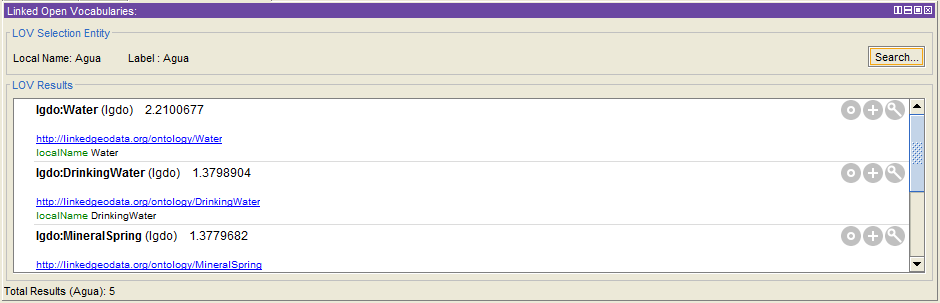
\includegraphics[scale=0.5]{img/LOVmockup.png}
%\label{fig:LOVresults}
%\caption{Panel showing the results for searching a term in the class hierarchy.}
%\end{figure}



